% MS-PI-CNNLSTM Architecture Diagram
% Compile with: pdflatex MS-PI-CNNLSTM_architecture.tex
% Requires: tikz, amsmath, amssymb
% Libraries: positioning, fit, arrows.meta, backgrounds, calc

\documentclass[border=3pt]{standalone}
\usepackage{tikz}
\usepackage{amsmath,amssymb}
\usetikzlibrary{positioning,fit,arrows.meta,backgrounds,calc}

\begin{document}
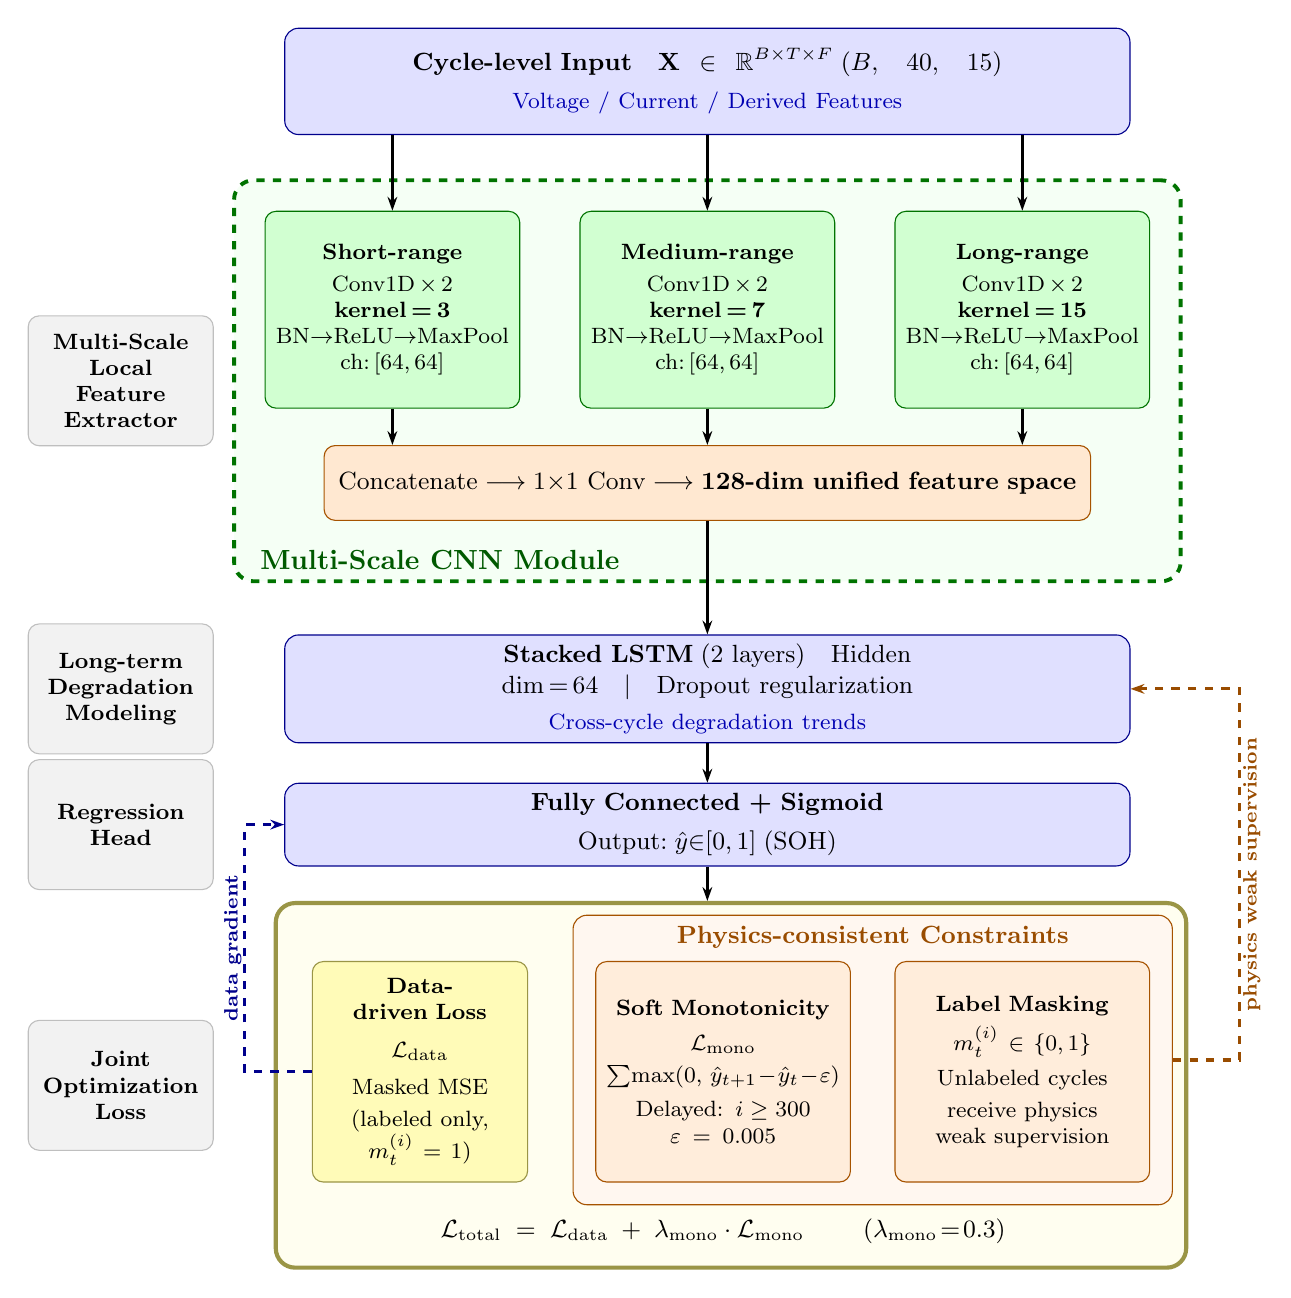
\begin{tikzpicture}[
  %% ── Block styles ──────────────────────────────────────────
  blueblock/.style={
    rounded corners=5pt,
    draw=blue!55!black, fill=blue!12,
    align=center, font=\small,
    text width=#1, minimum height=1.25cm
  },
  blueblock/.default=10.5cm,
  %
  greenblock/.style={
    rounded corners=4pt,
    draw=green!45!black, fill=green!18,
    align=center, font=\footnotesize,
    text width=3.0cm, minimum height=2.5cm
  },
  %
  concatblock/.style={
    rounded corners=4pt,
    draw=orange!65!black, fill=orange!18,
    align=center, font=\small,
    text width=9.5cm, minimum height=0.95cm
  },
  %
  ldatablock/.style={
    rounded corners=4pt,
    draw=yellow!55!black, fill=yellow!28,
    align=center, font=\footnotesize,
    text width=2.5cm, minimum height=2.8cm
  },
  %
  physblock/.style={
    rounded corners=4pt,
    draw=orange!65!black, fill=orange!14,
    align=center, font=\footnotesize,
    text width=3.0cm, minimum height=2.8cm
  },
  %
  sidelabel/.style={
    rounded corners=4pt,
    draw=gray!50, fill=gray!10,
    align=center, font=\footnotesize\bfseries,
    text width=2.05cm,
    minimum width=2.35cm,
    minimum height=1.65cm
  },
  %% ── Arrow styles ──────────────────────────────────────────
  fw/.style={
    -{Stealth[length=5pt,width=3.5pt]},
    line width=1.1pt
  },
  fbd/.style={
    -{Stealth[length=5pt,width=3.5pt]},
    line width=1.1pt, dashed,
    draw=blue!55!black
  },
  fbp/.style={
    -{Stealth[length=5pt,width=3.5pt]},
    line width=1.1pt, dashed,
    draw=orange!60!black
  },
]

%% ════════════════════════════════════════════════════════════
%% TITLE
%% ════════════════════════════════════════════════════════════
%% ════════════════════════════════════════════════════════════
%% INPUT BLOCK
%% ════════════════════════════════════════════════════════════
\node[blueblock, minimum height=1.35cm] (IN) at (0, 0) {
  \textbf{Cycle-level Input}\quad
  $\mathbf{X}\!\in\!\mathbb{R}^{B\times T\times F}$\;$(B,\;40,\;15)$\\[3pt]
  {\color{blue!70!black}\footnotesize Voltage / Current / Derived Features}
};

%% ════════════════════════════════════════════════════════════
%% THREE PARALLEL CNN BRANCHES
%% ════════════════════════════════════════════════════════════
\node[greenblock] (B1) at (-4.0, -2.9) {
  \textbf{Short-range}\\[2pt]
  Conv1D\,$\times$\,2\\
  \textbf{kernel\,=\,3}\\
  BN$\to$ReLU$\to$MaxPool\\
  ch:\,[64,\,64]
};

\node[greenblock] (B2) at (0, -2.9) {
  \textbf{Medium-range}\\[2pt]
  Conv1D\,$\times$\,2\\
  \textbf{kernel\,=\,7}\\
  BN$\to$ReLU$\to$MaxPool\\
  ch:\,[64,\,64]
};

\node[greenblock] (B3) at (4.0, -2.9) {
  \textbf{Long-range}\\[2pt]
  Conv1D\,$\times$\,2\\
  \textbf{kernel\,=\,15}\\
  BN$\to$ReLU$\to$MaxPool\\
  ch:\,[64,\,64]
};

%% ════════════════════════════════════════════════════════════
%% CONCATENATE + 1×1 CONV
%% ════════════════════════════════════════════════════════════
\node[concatblock] (CAT) at (0, -5.1) {
  Concatenate\;$\longrightarrow$\;1$\times$1 Conv\;$\longrightarrow$%
  \;\textbf{128-dim unified feature space}
};

%% ════════════════════════════════════════════════════════════
%% MULTI-SCALE CNN DASHED CONTAINER
%% ════════════════════════════════════════════════════════════
\coordinate (MSCNN_LABEL_SPACE) at ($(CAT.south)+(0,-0.38)$);
\begin{scope}[on background layer]
  \node[
    draw=green!45!black, fill=green!4,
    dashed, line width=1.4pt,
    rounded corners=7pt, inner sep=11pt,
    fit=(B1)(B2)(B3)(CAT)(MSCNN_LABEL_SPACE)
  ] (MSCNN) {};
\end{scope}

\node[
  font=\normalsize\bfseries,
  text=green!35!black,
  anchor=south west,
  inner sep=2pt
] at ($(MSCNN.south west)+(0.28,0.10)$) {Multi-Scale CNN Module};

%% ════════════════════════════════════════════════════════════
%% STACKED LSTM
%% ════════════════════════════════════════════════════════════
\node[blueblock, below=0.65cm of MSCNN] (LSTM) {
  \textbf{Stacked LSTM}\;(2 layers)\quad
  Hidden dim\,=\,64\quad$|$\quad Dropout regularization\\[2pt]
  {\color{blue!70!black}\footnotesize Cross-cycle degradation trends}
};

%% ════════════════════════════════════════════════════════════
%% FULLY CONNECTED + SIGMOID
%% ════════════════════════════════════════════════════════════
\node[blueblock, minimum height=1.05cm, below=0.5cm of LSTM] (FC) {
  \textbf{Fully Connected + Sigmoid}\\[3pt]
  Output:\;$\hat{y}{\in}[0,1]$\;(SOH)
};

%% ════════════════════════════════════════════════════════════
%% LOSS BOX CONTENTS
%% ════════════════════════════════════════════════════════════
%% --- Data-driven Loss ---
\node[ldatablock, anchor=north] (LDATA)
  at ($(FC.south)+(-3.65,-1.2)$) {
  \textbf{Data-driven Loss}\\[4pt]
  $\mathcal{L}_{\mathrm{data}}$\\[4pt]
  Masked MSE\\[2pt]
  (labeled only,\\
  $m_t^{(i)}\!=\!1$)
};

%% --- Soft Monotonicity Constraint ---
\node[physblock, anchor=north] (LMONO)
  at ($(FC.south)+(0.2,-1.2)$) {
  \textbf{Soft Monotonicity}\\[3pt]
  $\mathcal{L}_{\mathrm{mono}}$\\[2pt]
  $\sum\!\max(0,\,\hat{y}_{t+1}\!-\!\hat{y}_t\!-\!\varepsilon)$\\[3pt]
  Delayed: $i\!\geq\!300$\\
  $\varepsilon\!=\!0.005$
};

%% --- Label Masking ---
\node[physblock, anchor=north] (WMASK)
  at ($(FC.south)+(4.0,-1.2)$) {
  \textbf{Label Masking}\\[3pt]
  $m_t^{(i)}\!\in\!\{0,1\}$\\[3pt]
  Unlabeled cycles\\[2pt]
  receive physics\\
  weak supervision
};

\coordinate (PHYS_TITLE_SPACE) at ($(LMONO.north)+(0,0.30)$);
\coordinate (LOSS_TOP_SPACE) at ($(PHYS_TITLE_SPACE)+(0,0.26)$);

%% --- L_total formula ---
\node[font=\small\bfseries, anchor=north] (LTOTAL)
  at ($(LMONO.south)+(0,-0.34)$) {
  $\mathcal{L}_{\mathrm{total}}\;=\;
   \mathcal{L}_{\mathrm{data}}\;+\;
   \lambda_{\mathrm{mono}}\cdot\mathcal{L}_{\mathrm{mono}}$%
  \qquad$(\lambda_{\mathrm{mono}}\!=\!0.3)$
};

%% --- Outer loss box ---
\begin{scope}[on background layer]
  \node[
    draw=yellow!55!black, fill=yellow!6, line width=1.5pt,
    rounded corners=7pt, inner xsep=13pt, inner ysep=5pt,
    fit=(LDATA)(LOSS_TOP_SPACE)(LMONO)(WMASK)(LTOTAL)
  ] (LOSSBOX) {};
\end{scope}

%% --- Physics sub-box ---
\begin{scope}[on background layer]
  \node[
    draw=orange!65!black, fill=orange!6,
    rounded corners=5pt, inner sep=8pt,
    fit=(PHYS_TITLE_SPACE)(LMONO)(WMASK)
  ] (PHYSBOX) {};
\end{scope}

\node[
  font=\small\bfseries,
  text=orange!60!black,
  anchor=north,
  inner sep=1pt
] at ($(PHYSBOX.north)+(0,-0.10)$) {Physics-consistent Constraints};

%% ════════════════════════════════════════════════════════════
%% SIDE LABELS
%% ════════════════════════════════════════════════════════════
\coordinate (SLX) at (-7.45,0);

\node[sidelabel, anchor=center]
  at (SLX |- MSCNN.center) (SL1) {
  Multi-Scale\\Local Feature\\Extractor
};

\node[sidelabel, anchor=center]
  at (SLX |- LSTM.center) (SL2) {
  Long-term\\Degradation\\Modeling
};

\node[sidelabel, anchor=center]
  at (SLX |- FC.center) (SL3) {
  Regression\\Head
};

\node[sidelabel, anchor=center]
  at (SLX |- LOSSBOX.center) (SL4) {
  Joint\\Optimization\\Loss
};

%% ════════════════════════════════════════════════════════════
%% FORWARD FLOW ARROWS
%% ════════════════════════════════════════════════════════════
%% Input → three branches (fan out)
\coordinate (B1IN) at (B1.north);
\coordinate (B3IN) at (B3.north);
\coordinate (INL) at (B1IN |- IN.south);
\coordinate (INR) at (B3IN |- IN.south);
\draw[fw] (INL) -- (B1IN);
\draw[fw] (IN.south) -- (B2.north);
\draw[fw] (INR) -- (B3IN);

%% Branches → concat (fan in)
\coordinate (CATL) at ($(CAT.north)+(-4.0,0)$);
\coordinate (CATR) at ($(CAT.north)+( 4.0,0)$);
\draw[fw] (B1.south) -- (CATL);
\draw[fw] (B2.south) -- (CAT.north);
\draw[fw] (B3.south) -- (CATR);

%% Main vertical flow
\draw[fw] (CAT.south)   -- (LSTM.north);
\draw[fw] (LSTM.south)  -- (FC.north);
\coordinate (LOSSIN) at (FC.south |- LOSSBOX.north);
\draw[fw] (FC.south)    -- (LOSSIN);

%% ════════════════════════════════════════════════════════════
%% FEEDBACK ARROWS  (dashed, colored)
%% ════════════════════════════════════════════════════════════
%% Data gradient:  LDATA → FC  (left-side detour)
\draw[fbd]
  (LDATA.west)
    -- ++(-0.85, 0) coordinate (fdl)
    -- (fdl |- FC.west)
    -- (FC.west);
\node[font=\scriptsize\bfseries, text=blue!55!black, rotate=90, anchor=south, inner sep=1pt]
  at ($(fdl)!0.5!(fdl |- FC.west)$) {data gradient};

%% Physics weak supervision:  PHYSBOX → LSTM  (right-side detour)
\draw[fbp]
  (PHYSBOX.east)
    -- ++(0.85, 0) coordinate (fpr)
    -- (fpr |- LSTM.east)
    -- (LSTM.east);
\node[font=\scriptsize\bfseries, text=orange!60!black, rotate=90, anchor=north, inner sep=1pt]
  at ($(fpr)!0.5!(fpr |- LSTM.east)$) {physics weak supervision};

\end{tikzpicture}
\end{document}
